
\begin{multicols*}{2}

\section{Thief}

\lettrine[lines=3, lhang=0.15, loversize=0.25, findent=.5em]{T}{hieves} are experts at stealth and surprise, they can move through the shadows, vanish into thin air, or steal items from their opponents in the blink of an eye. 

\subsection*{Sneak Attack}

Beginning at 1st level, you know how to strike subtly and exploit a foe’s distraction. Once per turn, you can deal an extra 1d6 damage to one creature you hit with an attack if you have advantage on the attack roll. The attack must use a finesse or a ranged weapon.

You don’t need advantage on the attack roll if another enemy of the target is within 5 feet of it, that enemy isn’t incapacitated, and you don’t have disadvantage on the attack roll.

The amount of the extra damage increases as you gain levels in this class, as shown in the table below.

\header{Sneak attack damage}
\begin{rpg-table}
   	\textbf{Level}  & \textbf{Sneak Attack} \\
   	1st  & 1d6 \\
   	2nd  & 1d6 \\
    3rd  & 2d6 \\
    4th  & 2d6 \\
    5th  & 3d6 \\
    6th  & 3d6 \\
    7th  & 4d6 \\
    8th  & 4d6 \\
    9th  & 5d6 \\
    10th & 5d6 \\
\end{rpg-table}




\subsection*{Cunning Action}

At 3rd level, you learn maneuvers that are fueled by your cunning dice. Refer to the rogue's cunning action table for details.

\subsection*{Etheral Jaunt}

You are a master of subterfuge. At 5th level, you can see normally in darkness, both magical and nonmagical, to a distance of 30 feet.

Additionally, you gain the ability to step from one shadow into another. When you are in dim light or darkness, as a bonus action you can teleport up to 60 feet to an unoccupied space you can see that is also in dim light or darkness. The teleport action is either of magical nature or raw physical reflexes. 

You can use this feature three times. You regain all expended uses of it when you finish a long rest. You can burn cunning point for additional uses.

\subsection*{Pierce the Veil}

Like a ghost, you have the ability to slip in and out of the Ethereal Plane.

Starting at the 9th level, you can use your cunning action in your first turn of a combat to cast the blink spell.

Once you use this feature, you can’t use it again until you finish a long rest or until you spend a spell slot of 3rd level or higher.

\begin{Figure}
\centering
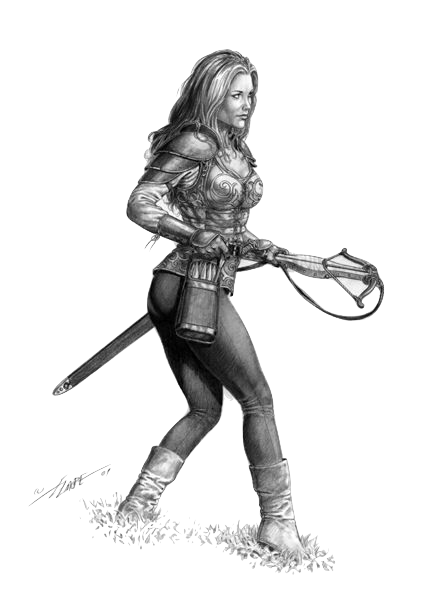
\includegraphics[width=\textwidth]{img/female-rogue.png}
{\scriptsize Art by Larry Elmore}
\end{Figure}
    
\end{multicols*}


\clearpage

\begin{table}[ht!]
\begin{small}
\rowcolors{2}{}{commentgreen}
\begin{center}
\begin{tabular}{ll}
\multicolumn{2}{l}{\parbox[l][0.6cm][c]{15cm}{\textbf{Rogue Cunning Actions}}} 
\\
\hline 
\textbf{Name} & \parbox[l][0.6cm][c]{15cm}{\textbf{Description}}
\\ 
Quick Footwork & \parbox[l][1.8cm][c]{15cm}{
Your quick thinking and agility allow you to move and act quickly. You can spend one cunning point to take a bonus action on each of your turns in combat. This action can be used only to take the Dash, Disengage, or Hide action.
}
\\ 
Quick Reflexes & \parbox[l][1.2cm][c]{15cm}{
You can spend one cunning point to take the Dodge action as a bonus action on your turn.
}
\\ 
Fast Hands & \parbox[l][1.8cm][c]{15cm}{
You can spend one cunning point and use your bonus action to make a Dexterity (Sleight of Hand) check, use your thieves' tools to disarm a trap or open a lock, or take the Use an Object action.
}
\\
Precision Attack & \parbox[l][1.8cm][c]{15cm}{
When you make a weapon attack roll against a creature, you can expend one cunning die to add it to the roll. You can use this maneuver before or after making the attack roll, but before any effects of the attack are applied.
}
\\
Slow Fall & \parbox[l][1.2cm][c]{15cm}{
You can use your reaction when you fall to spend one cunning point and reduce any falling damage you take by an amount equal to five times your cunning die.
}
\\
\hline
\end{tabular}
\end{center}
\end{small}
\end{table}    

